% Compile with: pdflatex mindmap.tex
\documentclass[border=15mm]{standalone}
\usepackage[T1]{fontenc}
\usepackage{lmodern}
\usepackage{tikz}
\usetikzlibrary{mindmap,backgrounds,positioning}

% --- Color palette (9 branches) ---
\definecolor{coreColor}{HTML}{495057}
\definecolor{brA}{HTML}{E8590C}  % Orange  - VAEs & Autoencoders
\definecolor{brB}{HTML}{1971C2}  % Blue    - Diffusion Models
\definecolor{brC}{HTML}{2F9E44}  % Green   - Graph-Based Generation
\definecolor{brD}{HTML}{9C36B5}  % Purple  - Corrosion Prediction
\definecolor{brE}{HTML}{E67700}  % Amber   - UV & Optical Prediction
\definecolor{brF}{HTML}{0CA678}  % Teal    - Mechanical Prediction
\definecolor{brG}{HTML}{D6336C}  % Pink    - Bayesian Optimization
\definecolor{brH}{HTML}{4263EB}  % Indigo  - Active Learning
\definecolor{brI}{HTML}{1098AD}  % Cyan    - Multi-Objective Optimization

\begin{document}
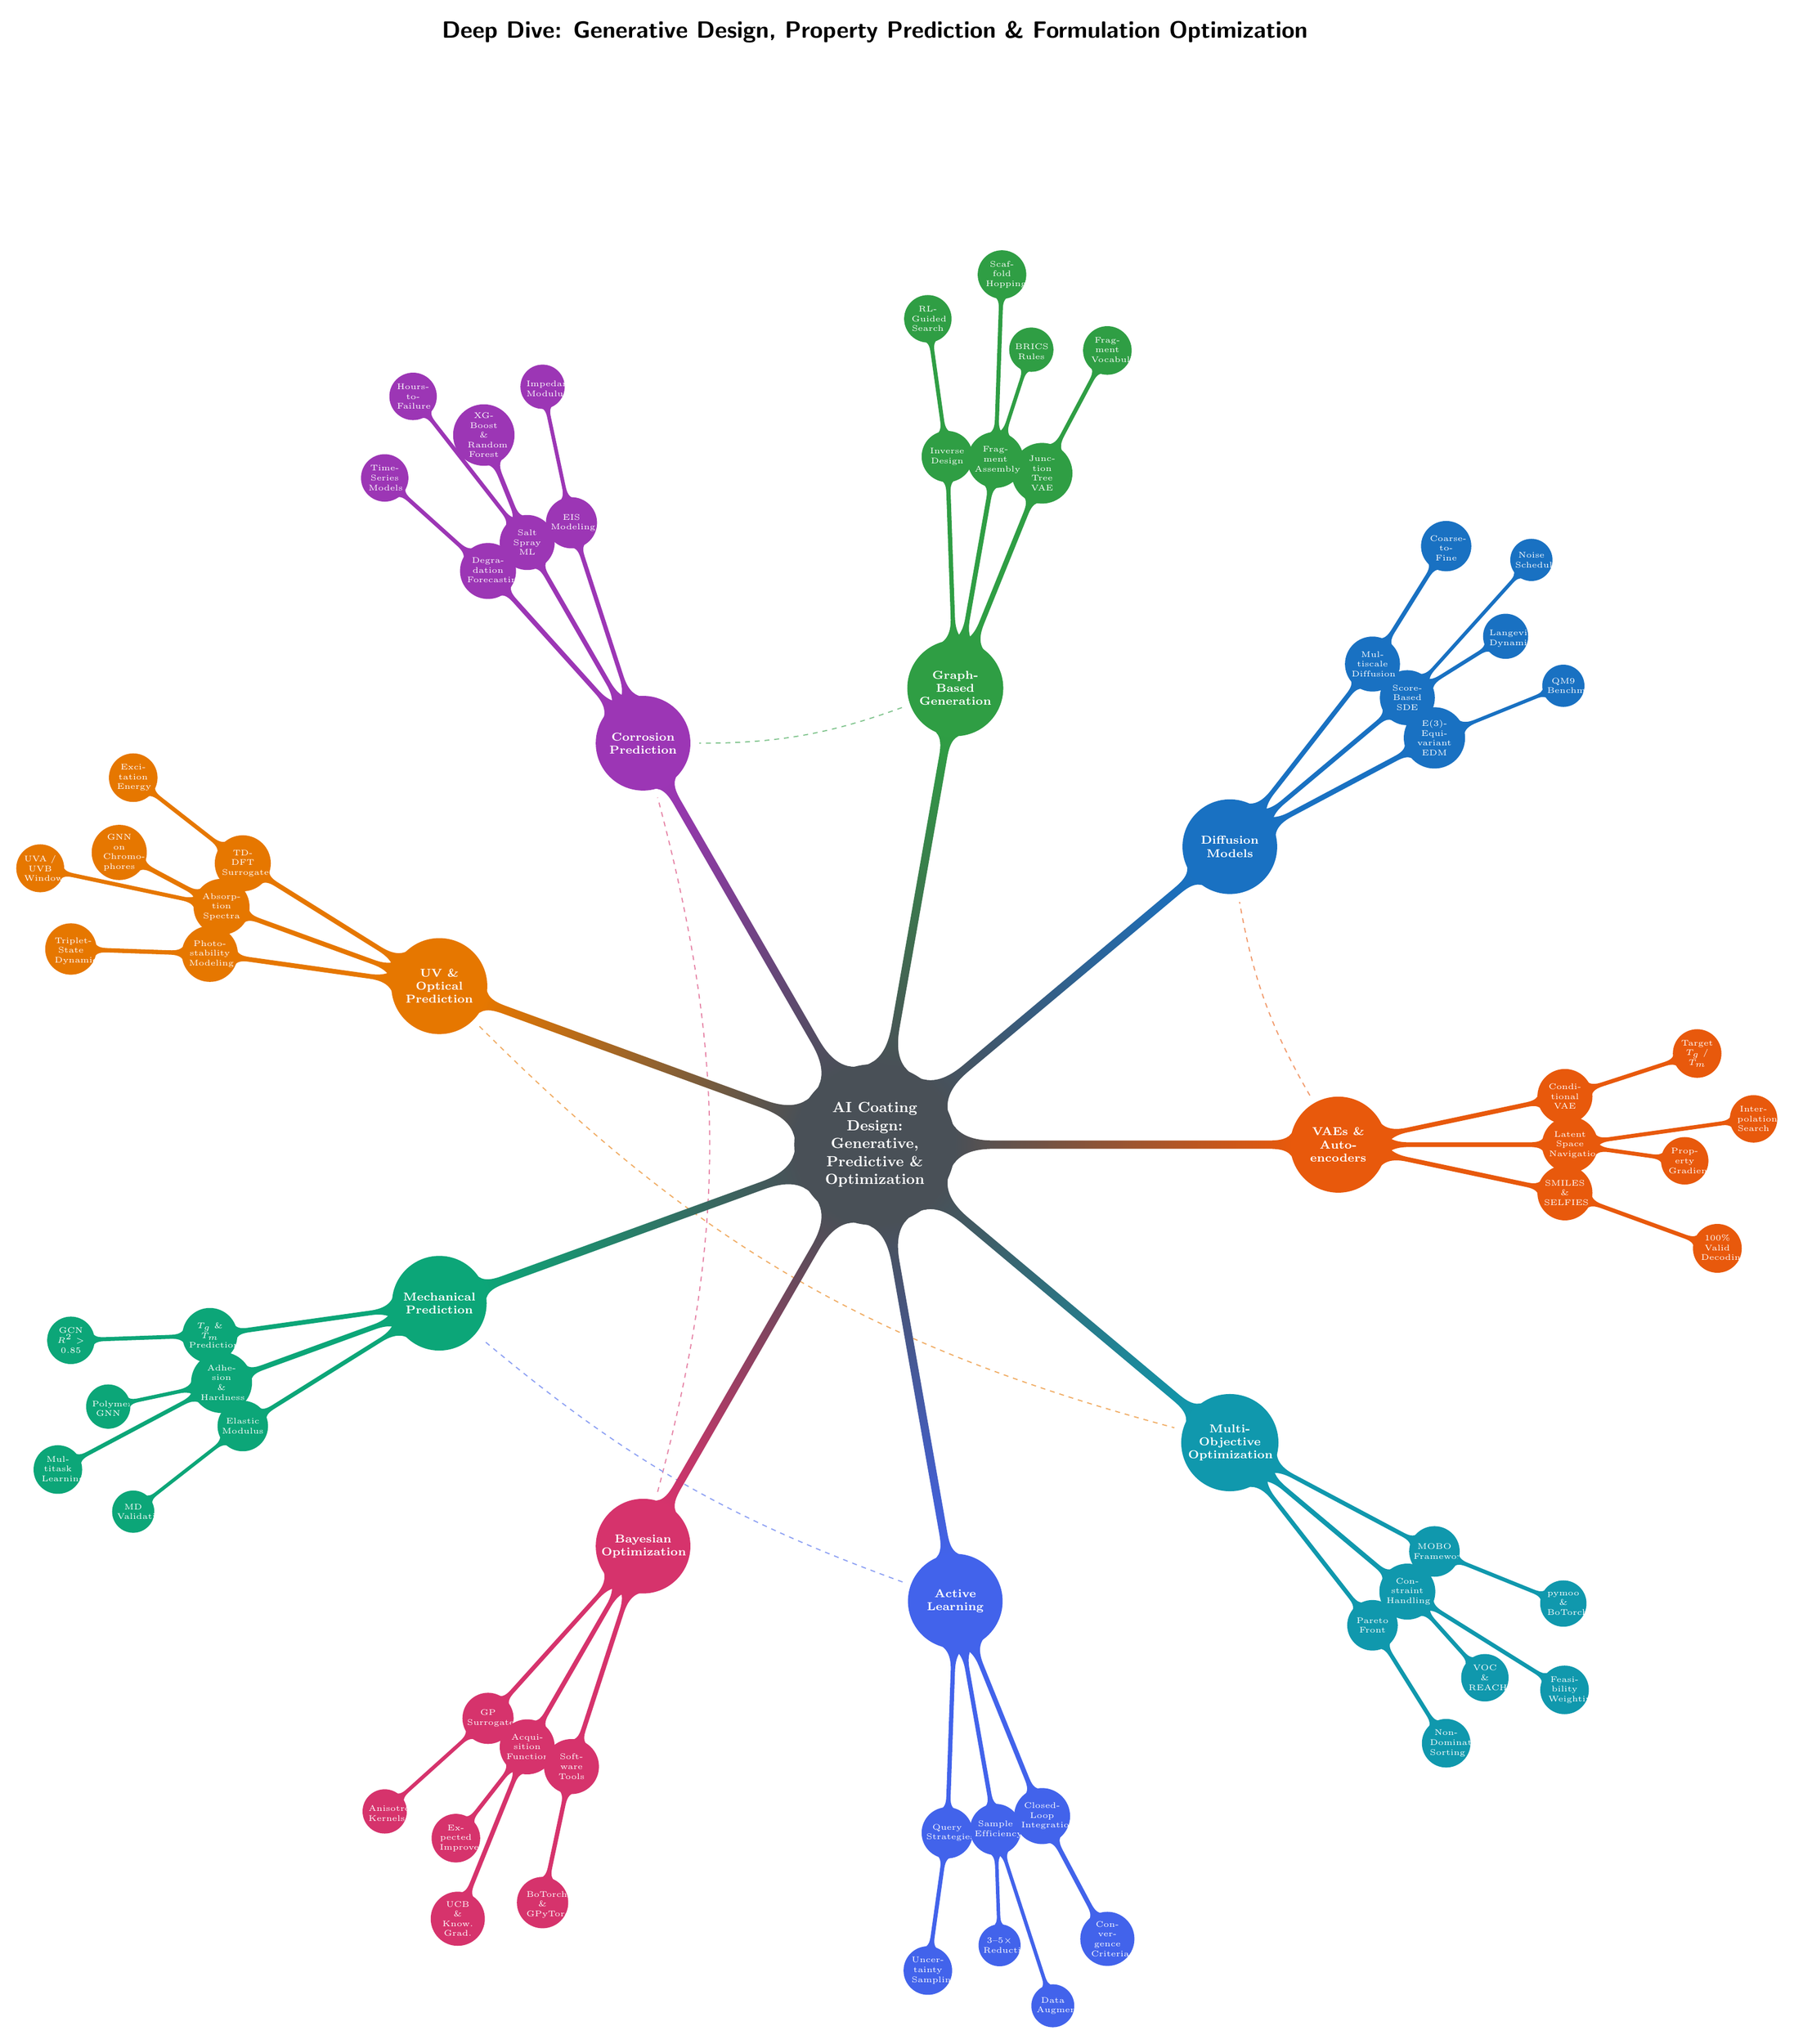
\begin{tikzpicture}

% --- Title ---
\node[font=\Large\bfseries\sffamily] at (0,24)
  {Deep Dive: Generative Design, Property Prediction \& Formulation Optimization};

\begin{scope}[
  mindmap,
  every node/.style={concept, execute at begin node=\hskip0pt},
  grow cyclic,
  text=white,
  concept color=coreColor,
  level 1/.append style={
    level distance=10cm, sibling angle=40,
    font=\scriptsize\bfseries, minimum size=2.0cm, text width=1.8cm,
  },
  level 2/.append style={
    level distance=5.0cm, sibling angle=12,
    font=\tiny, minimum size=1.0cm, text width=0.9cm,
  },
  level 3/.append style={
    level distance=4.0cm, sibling angle=25,
    font=\tiny, minimum size=0.8cm, text width=0.7cm,
  },
]

\node [font=\small\bfseries, minimum size=3.2cm, text width=2.8cm]
  (center) {AI Coating\\Design:\\Generative,\\Predictive \&\\Optimization}
%
% ===== Branch 1: VAEs & Autoencoders (0 deg) =====
  child [concept color=brA, grow=0] {
    node (vaes) {VAEs \&\\Auto\-encoders}
    child [grow=-12] {
      node {SMILES \&\\SELFIES}
      child [grow=-20, level distance=3.5cm] { node {100\%\\Valid\\Decoding} }
    }
    child [grow=0] {
      node {Latent Space\\Navigation}
      child [grow=-8, level distance=2.5cm] { node {Property\\Gradient} }
      child [grow=8, level distance=4.0cm] { node {Inter\-polation\\Search} }
    }
    child [grow=12] {
      node {Conditional\\VAE}
      child [grow=18, level distance=3.0cm] { node {Target\\$T_g$ / $T_m$} }
    }
  }
%
% ===== Branch 2: Diffusion Models (40 deg) =====
  child [concept color=brB, grow=40] {
    node (diffusion) {Diffusion\\Models}
    child [grow=28] {
      node {E(3)-Equi\-variant\\EDM}
      child [grow=22, level distance=3.0cm] { node {QM9\\Benchmark} }
    }
    child [grow=40] {
      node {Score-Based\\SDE}
      child [grow=32, level distance=2.5cm] { node {Langevin\\Dynamics} }
      child [grow=48, level distance=4.0cm] { node {Noise\\Schedule} }
    }
    child [grow=52] {
      node {Multiscale\\Diffusion}
      child [grow=58, level distance=3.0cm] { node {Coarse-to-\\Fine} }
    }
  }
%
% ===== Branch 3: Graph-Based Generation (80 deg) =====
  child [concept color=brC, grow=80] {
    node (graphgen) {Graph-Based\\Generation}
    child [grow=68] {
      node {Junction\\Tree VAE}
      child [grow=62, level distance=3.0cm] { node {Fragment\\Vocabulary} }
    }
    child [grow=80] {
      node {Fragment\\Assembly}
      child [grow=72, level distance=2.5cm] { node {BRICS\\Rules} }
      child [grow=88, level distance=4.0cm] { node {Scaffold\\Hopping} }
    }
    child [grow=92] {
      node {Inverse\\Design}
      child [grow=98, level distance=3.0cm] { node {RL-Guided\\Search} }
    }
  }
%
% ===== Branch 4: Corrosion Prediction (120 deg) =====
  child [concept color=brD, grow=120] {
    node (corrpred) {Corrosion\\Prediction}
    child [grow=108] {
      node {EIS\\Modeling}
      child [grow=102, level distance=3.0cm] { node {Impedance\\Modulus} }
    }
    child [grow=120] {
      node {Salt Spray\\ML}
      child [grow=112, level distance=2.5cm] { node {XGBoost \&\\Random Forest} }
      child [grow=128, level distance=4.0cm] { node {Hours-to-\\Failure} }
    }
    child [grow=132] {
      node {Degradation\\Forecasting}
      child [grow=138, level distance=3.0cm] { node {Time-Series\\Models} }
    }
  }
%
% ===== Branch 5: UV & Optical Prediction (160 deg) =====
  child [concept color=brE, grow=160] {
    node (uvpred) {UV \&\\Optical\\Prediction}
    child [grow=148] {
      node {TD-DFT\\Surrogates}
      child [grow=142, level distance=3.0cm] { node {Excitation\\Energy} }
    }
    child [grow=160] {
      node {Absorption\\Spectra}
      child [grow=152, level distance=2.5cm] { node (gnnchrom) {GNN on\\Chromo\-phores} }
      child [grow=168, level distance=4.0cm] { node {UVA / UVB\\Windows} }
    }
    child [grow=172] {
      node {Photo\-stability\\Modeling}
      child [grow=178, level distance=3.0cm] { node {Triplet-State\\Dynamics} }
    }
  }
%
% ===== Branch 6: Mechanical Prediction (200 deg) =====
  child [concept color=brF, grow=200] {
    node (mechpred) {Mechanical\\Prediction}
    child [grow=188] {
      node {$T_g$ \& $T_m$\\Prediction}
      child [grow=182, level distance=3.0cm] { node {GCN\\$R^2 > 0.85$} }
    }
    child [grow=200] {
      node {Adhesion \&\\Hardness}
      child [grow=192, level distance=2.5cm] { node {Polymer\-GNN} }
      child [grow=208, level distance=4.0cm] { node {Multitask\\Learning} }
    }
    child [grow=212] {
      node {Elastic\\Modulus}
      child [grow=218, level distance=3.0cm] { node {MD\\Validation} }
    }
  }
%
% ===== Branch 7: Bayesian Optimization (240 deg) =====
  child [concept color=brG, grow=240] {
    node (bayesopt) {Bayesian\\Optimization}
    child [grow=228] {
      node {GP\\Surrogates}
      child [grow=222, level distance=3.0cm] { node {Anisotropic\\Kernels} }
    }
    child [grow=240] {
      node {Acquisition\\Functions}
      child [grow=232, level distance=2.5cm] { node {Expected\\Improvement} }
      child [grow=248, level distance=4.0cm] { node {UCB \&\\Know.\ Grad.} }
    }
    child [grow=252] {
      node {Software\\Tools}
      child [grow=258, level distance=3.0cm] { node {BoTorch \&\\GPyTorch} }
    }
  }
%
% ===== Branch 8: Active Learning (280 deg) =====
  child [concept color=brH, grow=280] {
    node (activelearn) {Active\\Learning}
    child [grow=268] {
      node {Query\\Strategies}
      child [grow=262, level distance=3.0cm] { node {Uncertainty\\Sampling} }
    }
    child [grow=280] {
      node {Sample\\Efficiency}
      child [grow=272, level distance=2.5cm] { node {3--5$\times$\\Reduction} }
      child [grow=288, level distance=4.0cm] { node {Data\\Augmentation} }
    }
    child [grow=292] {
      node {Closed-Loop\\Integration}
      child [grow=298, level distance=3.0cm] { node {Convergence\\Criteria} }
    }
  }
%
% ===== Branch 9: Multi-Objective Optimization (320 deg) =====
  child [concept color=brI, grow=320] {
    node (moopt) {Multi-Objective\\Optimization}
    child [grow=308] {
      node {Pareto\\Front}
      child [grow=302, level distance=3.0cm] { node {Non-Dominated\\Sorting} }
    }
    child [grow=320] {
      node {Constraint\\Handling}
      child [grow=312, level distance=2.5cm] { node {VOC \&\\REACH} }
      child [grow=328, level distance=4.0cm] { node {Feasibility\\Weighting} }
    }
    child [grow=332] {
      node {MOBO\\Frameworks}
      child [grow=338, level distance=3.0cm] { node {pymoo \&\\BoTorch} }
    }
  }
;
\end{scope}

% --- Cross-branch connections ---
\begin{pgfonlayer}{background}
  % VAEs <-> Diffusion (shared latent-space paradigm)
  \draw [dashed, brA!60, line width=0.7pt, shorten >=6pt, shorten <=6pt]
    (vaes) to[bend left=10] (diffusion);
  % Graph Generation <-> Corrosion Prediction (screen generated molecules)
  \draw [dashed, brC!60, line width=0.7pt, shorten >=6pt, shorten <=6pt]
    (graphgen) to[bend left=10] (corrpred);
  % Bayesian Opt <-> EIS / Corrosion (BO drives experiment selection)
  \draw [dashed, brG!60, line width=0.7pt, shorten >=6pt, shorten <=6pt]
    (bayesopt) to[bend right=15] (corrpred);
  % UV Prediction <-> Multi-Objective (UV absorption as objective)
  \draw [dashed, brE!60, line width=0.7pt, shorten >=6pt, shorten <=6pt]
    (uvpred) to[bend right=15] (moopt);
  % Active Learning <-> Mechanical Pred (AL reduces data for mech. models)
  \draw [dashed, brH!60, line width=0.7pt, shorten >=6pt, shorten <=6pt]
    (activelearn) to[bend left=10] (mechpred);
\end{pgfonlayer}

\end{tikzpicture}
\end{document}
